\chapter{Algorithm optimization}
\label{chap:results}

We used henceforth classification performance as a proxy to neural representation. Since we want to understand how information about time develops in the brain during learning of the task, we compared this classification performance in the beginning of the session and near the end of the session. Before making this comparison, we tested multiple classifiers to be sure that any kind of information captured by then is not specific to the classifier.
\subsection{Classification}

\section{Rationale}
    \begin{figure}
        \centering
        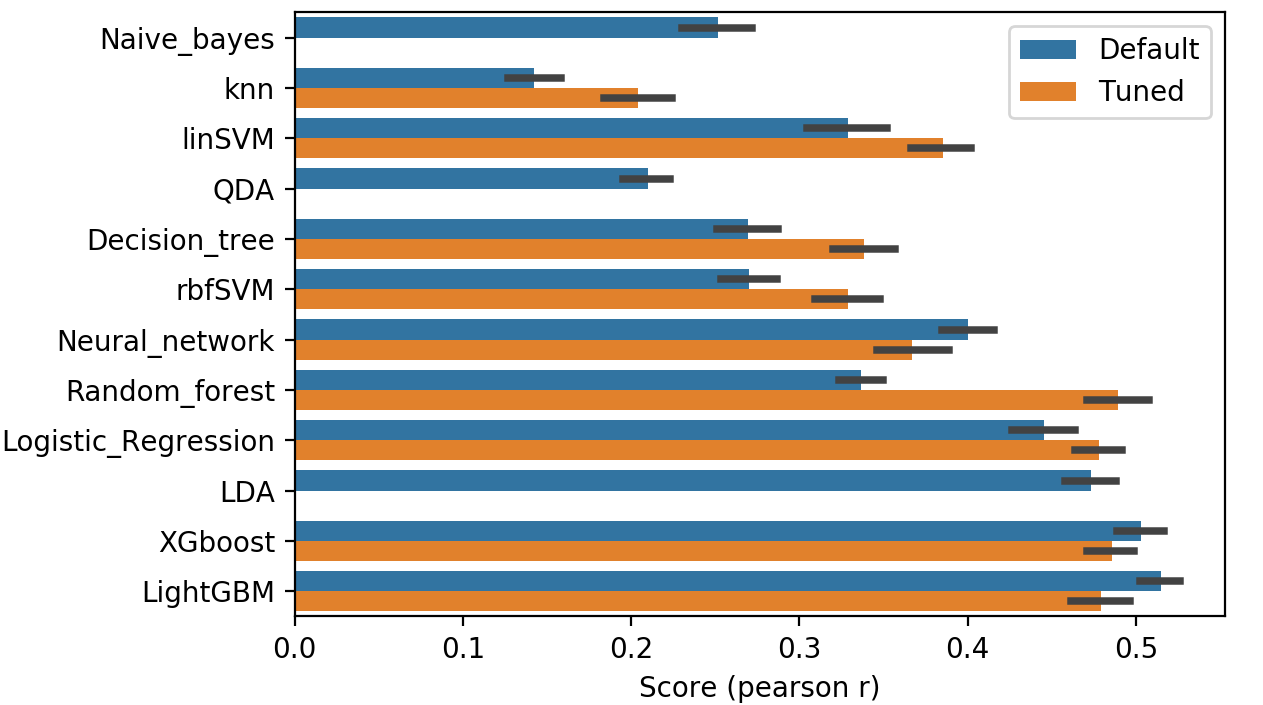
\includegraphics[width=\textwidth]{figures/hyperparameter_tuning_12_classifiers.png}
        \caption[Comparison of classifiers]{Comparison of classifiers. Default hyperparameters were compared with those resulting from tuning when there were hyperparameters to tune.}
        \label{fig:clf_comparison}
    \end{figure} % Mean performance+-SEM for each classifier tuned and untuned. 
    Firstly, we compared classification performances for different classifiers, in such a way as to make an informed choice for our subsequent analysis. We calculate scores in each tuning step with 5 folds of Monte Carlo cross validation, and evaluate the final scores with 50 folds. Half of the trials were hold out for tuning, trials from the other half were used for evaluation of the final score.
    
    We found big differences in performance between the multiple classifiers tested. Some classifiers have good results out-of-the-box, such as Logistic Regression and Linear Discriminant Analysis (LDA), while some are highly dependent on hyperparameter tuning, such as Random Forest. The results for the gradient boosting classifiers LightGBM and XGBoost are specially interesting, as they have better results on the default configurations than after tuning, which is probably due to the fact that we were tuning 10 different hyperparameters, making us prone to overfitting the tuning.
    
    \begin{figure}
        \centering
        % \includegraphics[width=\textwidth]{figuras/methods/learning_curves_sppfc.png}
        \caption{Classifier learning curves}
        \label{fig:clf_curves}
    \end{figure}
    % Colocar aqui somente para os melhores. Colocar os outros no material suplementar.
    For most classifiers, there is significant decoding for as little as 10 trials in the training set. As expected, the classifier's performance increases with the number of trials used for training it. It is even possible that a bigger training set would give us even higher scores, pointing to the importance of having big experimental sessions with many trials. Hence, if we want to compare the information contained in the neural activity in different moments in a session, we have to ensure their classification models are trained with the same number of trials.
